\begin{figure}
    \begin{center}
    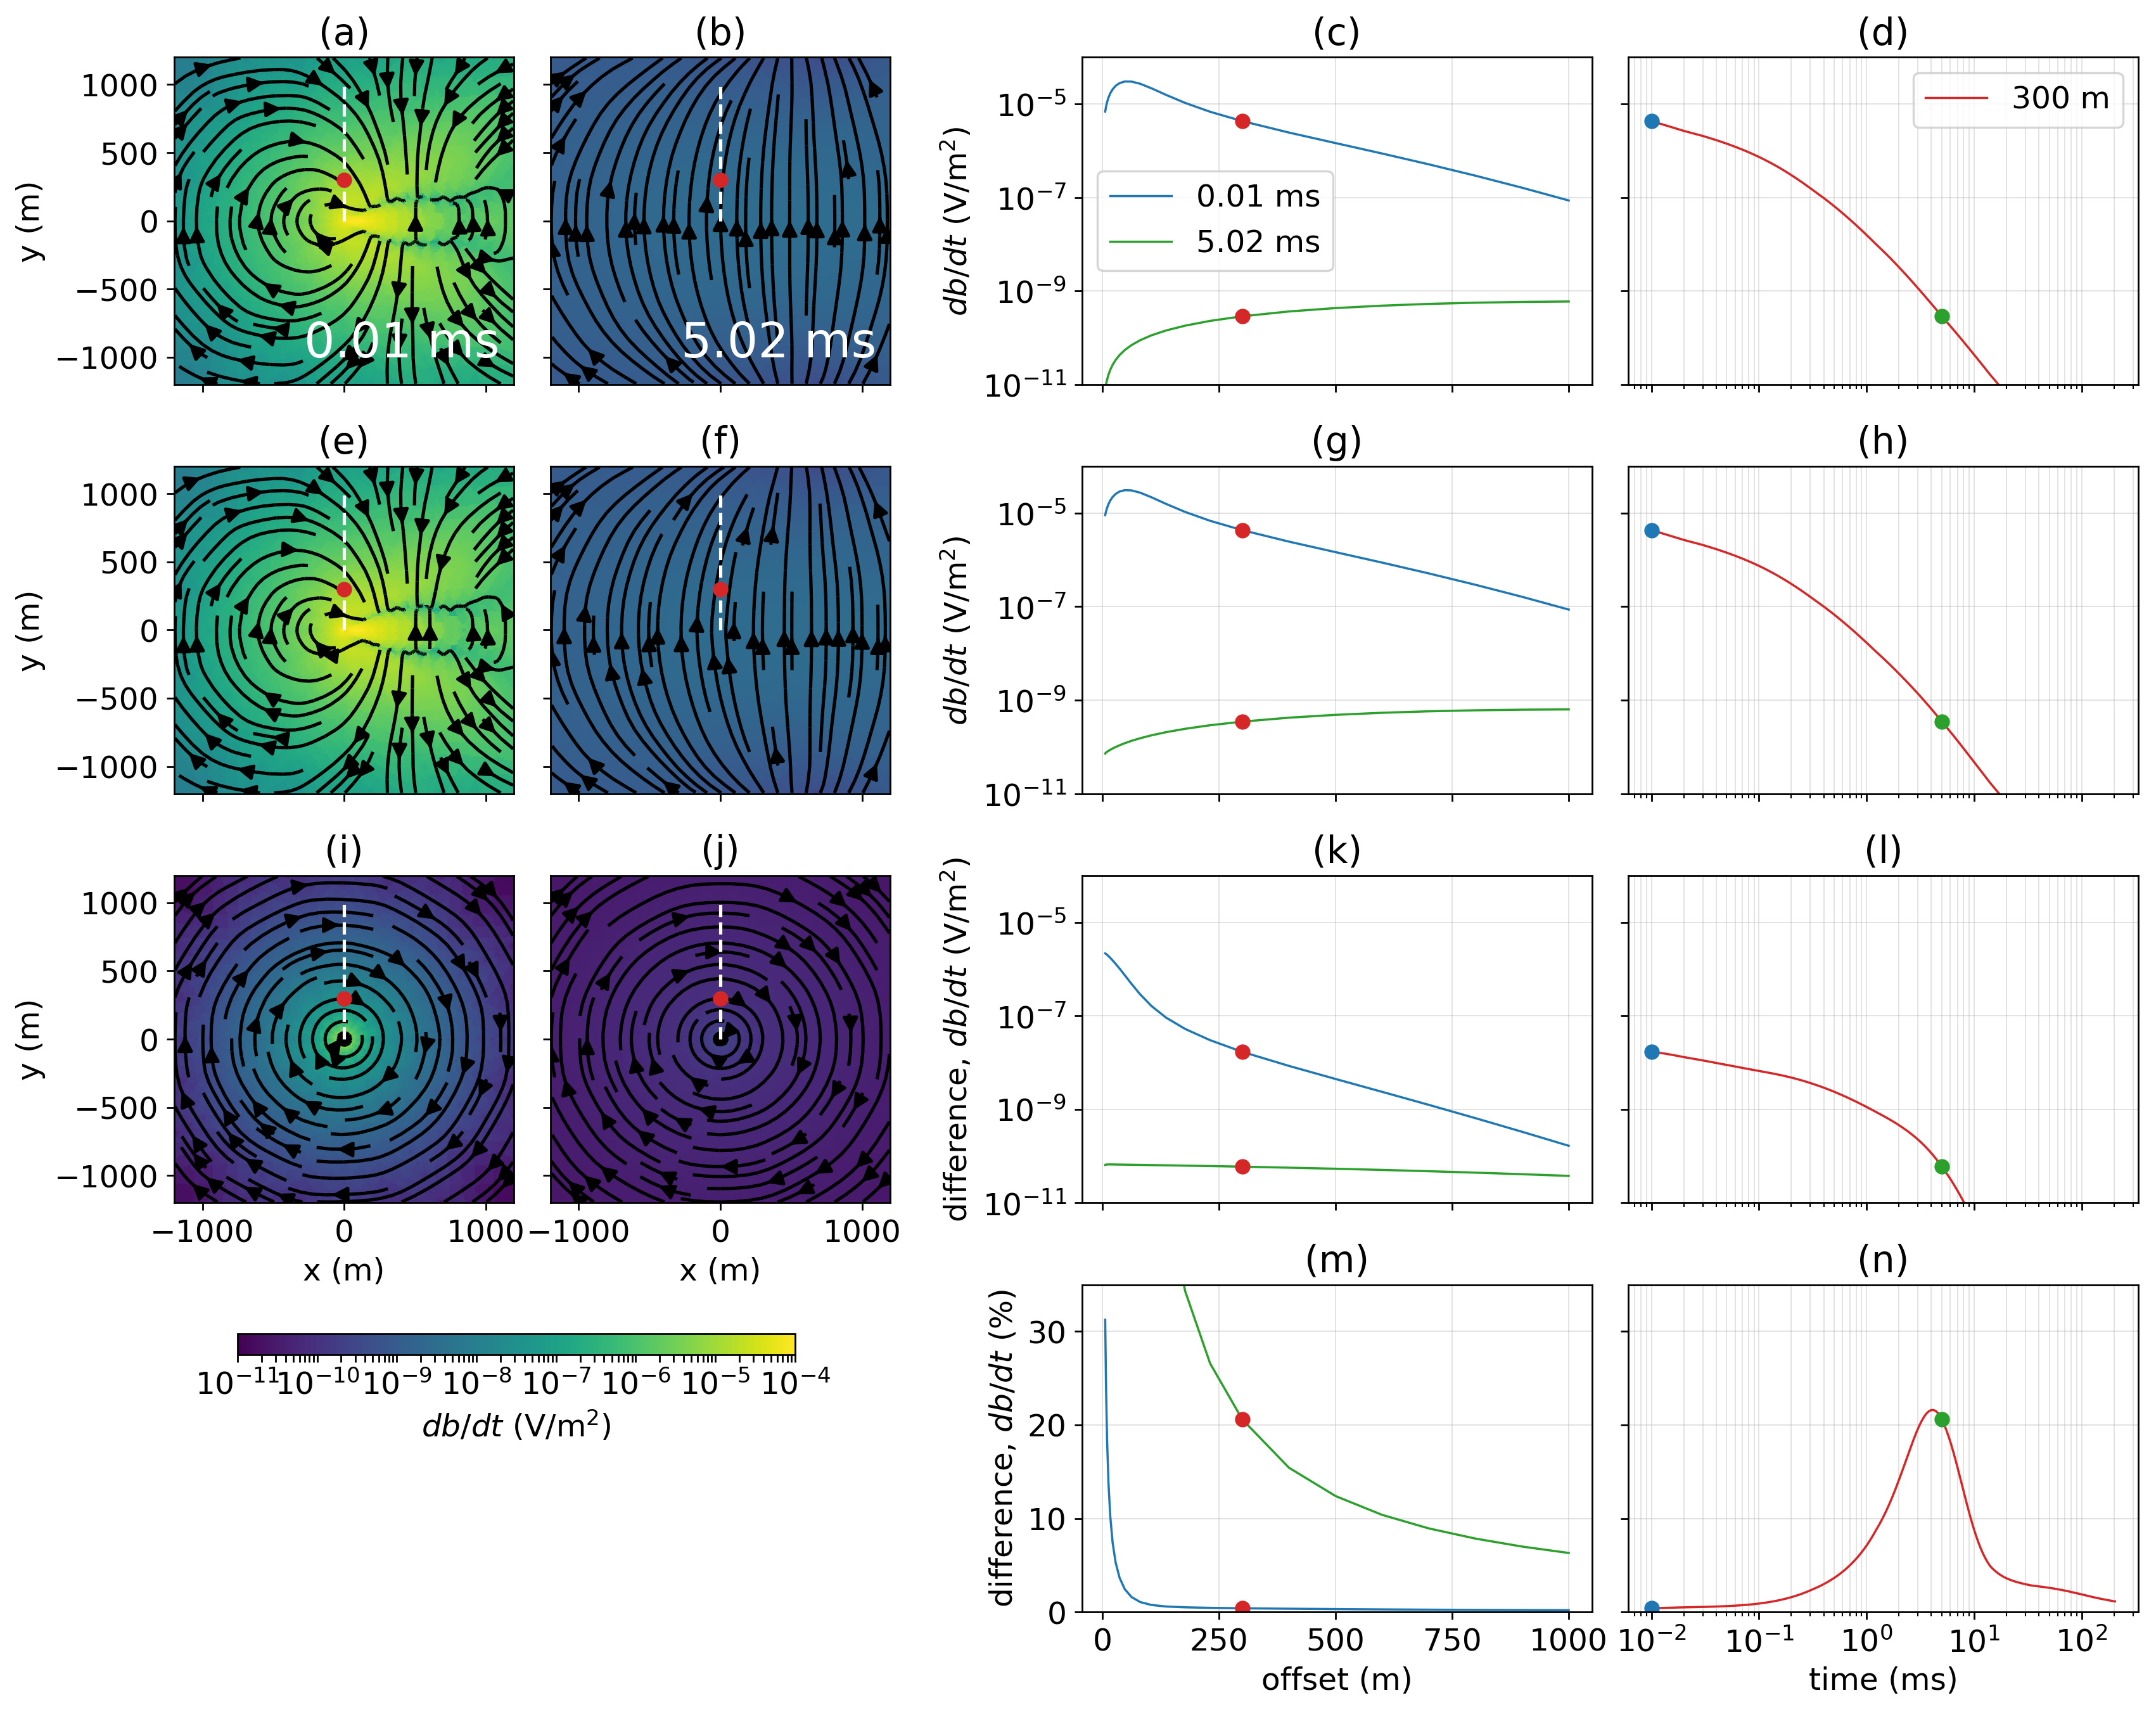
\includegraphics[width=\textwidth]{figures/em_casing/surface_dbdt_overview.png}
    \end{center}
\caption{
    Simulated $db/dt$ at (a) 0.01 ms and (b) 5 ms after shut-off for the halfspace model.
    (c) Tangential $db/dt$ measured along the white line in (a) and (b) at 0.01 ms (blue) and 5 ms (green).
    (d) Tangential $db/dt$ as a function of time at 300 m along the survey line (shown in the red dot in (a)).
    Similar information is shown in (e), (f), (g) and (h) for the model with the conductive casing.
    The difference in the $db/dt$ data (casing minus halfspace) is shown in (i), (j), (k) and (l).
    The difference is also shown as a percentage of the halfspace solution at 0.01 ms and 5 ms in (m)
    and through time at 300 m offset in (n).
}
\label{fig:surface_dbdt_overview}
\end{figure}



